\chapter{The Hybrid Fortran Framework} \label{cha:framework}
Hybrid Fortran is a directive based extension of the and a code transformation tool within the Fortran language. It is intended for enabling GPGPU acceleration of data parallel programs using a unified codebase. Performance Portability was a major design aspect of this framework - not only should it enable the accelerated target to achieve optimal performance, but the CPU target should keep performing as before the migration. In the backend it automatically creates CUDA Fortran or OpenACC Fortran code for GPU and OpenMP Fortran code for CPU, in both cases making use of data parallelism defined by the user through directives. Additionally, a GNU Make build system as well as an automatic test system is provided. Hybrid Fortran has been successfully used for speeding up the Physical Core of Japan's national next generation weather prediction model by a factor of 3.6x on Kepler K20x vs. 6 Core Westmere \textit{while not loosing any CPU performance}.

This chapter will describe the functionality of the \textbf{Hybrid Fortran} framework from a user perspective. Chapter \ref{cha:usage} guides through setup, portation, debugging and testing in a 'howto'-like fashion. Chapter \ref{cha:implementation} will go into implementation details for those who would like to adapt \textbf{Hybrid Fortran} to their own specific usecases.

\section{Design Goals} \label{sec:frameworkGoals}

This section gives an overview over the design goals of the \textbf{Hybrid Fortran} framework.

\begin{enumerate}
 \item \textbf{Hybrid Fortran} is intended to enable performance portable parallel programming for HPC purposes.
 \item \label{h90goals:unifiedCodebase} \textbf{Hybrid Fortran} offers a unified codebase for both CPU and GPU execution.

 \item \label{h90goals:compileTimeDefinedStorageOrder} The storage order is compile time defined since CPU and GPU implementations usually have different ideal storage orders.
 \item \label{h90goals:lowComplexity} The rules for creating the GPU code versions should have a low complexity, such that optimizations performed by the user lead to predictable results.
 \item \label{h90goals:performance} The framework enables GPU performance at the level of hand optimized CUDA Fortran while maintaining CPU performance as close as possible to the original CPU code.
 \item \label{h90goals:flexibleImplementation} The implementation details are abstracted from the rest of the system, such that other parallel programming frameworks can be supported in the future without changes in the user code.
 \item \textbf{Hybrid Fortran} is optimized for two use cases in particular: Stencil access patterns with tight loops and Parallel vector access patterns with outside loops. \textbf{Hybrid Fortran} abstracts domain specifications of arrays such that the migration path from typical Fortran code for these two use cases becomes minimal.
\end{enumerate}

\clearpage
\section{Features} \label{sec:features}
\begin{itemize}
 \item Backends for OpenACC (GPU), CUDA Fortran (GPU) and OpenMP (CPU) parallelizations.

 \item Separate parallel regions for CPU and GPU at multiple points in the callgraph (if needed). This allows high performance for both CPU and GPU implementations.

 \item Compile-time defined storage order with different orders for CPU and GPU - all defined in one handy place, the \verb|storage_order.F90| file. Multiple storage orders are supported through attributes in the Hybrid Fortran directives.

 \item Automatic compile time array reformatting - Hybrid Fortran reformats your data with respect to privatization and storage order at compile time. This means you can leave existing Fortran code as is, only the setup using the two Hybrid Fortran directives is needed.

 \item Temporary automatic arrays, module data and imported scalars within GPU kernels (aka subroutines containing a GPU `@parallelRegion`) - this functionality is provided in addition to CUDA Fortran's device syntax features.

 \item Support for Pointers.

 \item Separate build directories for the automatically created CPU and GPU codes, showing you the created F90 files. Get a clear view of what happens in the back end without cluttering up your source directories.

 \item Use any x86 Fortran compiler for the CPU code (PGI and Intel Fortran have been tested).

 \item Highly human readable intermediate F90 source files. The callgraph, including subroutine names, remains the same as in the user code you specify. The code in the intermediate source files is auto indented for additional reading comfort.

 \item Macro support for your codebase - a separate preprocessor stage is applied even before the hybrid fortran preprocessor comes in, in order to facilitate the DRY principle.

 \item Arbitrary usage of line length and line continuations is allowed in Hybrid Fortran. The framework will automatically merge all continued lines, then apply the transformation steps, then split the lines up again in order to ensure compliance with Fortran compilers.

 \item Automatic creation of your callgraph as a graphviz image, facilitating your code reasoning. Simply type `make graphs` in the command line in your project directory.

 \item Automatic testing together with your builds - after an initial setup you can run validation tests as well as valgrind automatically after every build (or by running `make tests`). As an example, say you'd like the preprocessor to tell you that there is a calculation error in array X at point i=10,j=5,k=3? If you set up everything accordingly, this is pretty much what Hybrid Fortran does for you. This speeds up development in large framework a lot, since automated testing means that you can check your work after each submodule or even kernel.

 \item Automatic 'printf' based device debugging mode. Prints all input arrays, output arrays and temporary arrays at the end of each kernel run at a compile-time specified point in a nicely readable format. This output can then be manually validated against the CPU version (which should already produce correct results at that point). Please note: Since PGI's CUDA Fortran does not yet support real device debugging, Hybrid Fortran cannot support that either at this point. However, since the code runs on CPU as well, the class of bugs that are affected by this restriction is rather small (since computational code can be validated on the CPU first) and the current debug mode has been proven to be sufficient for the time being.

 \item Automatic linking and installing of executables. Simply specify the executable names in the `MakesettingsGeneral` configuration file and use corresponding filenames for the main files (which can be placed anywhere in your source tree). The Hybrid Fortran build system will automatically generate the executables (each in CPU and GPU version) and install them in subdirectories of your test directory. The test directories are persistant, such that you can put your initialization files, validation scripts and performance test scripts there. All this happens simply through running `make; make install` in your project directory.
\end{itemize}

\clearpage
\section{Hybrid Fortran Directives} \label{sec:archDirectives}

The directives introduced with the \textbf{Hybrid Fortran} framework are the only additions that have been made to the Fortran 90 language in order to achieve the objectives stated in sec.~\ref{sec:frameworkGoals}. All other syntax elements in \textbf{Hybrid Fortran} are a strict subset of Fortran 90.

It is necessary to introduce the following denotations before introducing the new directives:

\begin{description}
 \item [A domain] in this context denotes a tuple containing a data dimension and its size. For example, if we have an array \verb|a| declared within the range $(1,\unit{NX})$ and looped over using the iterator \verb|x|, we call this array to be \textbf{domain dependant} in domain \verb|x|. For simplicity, we assume that iterators over the same data dimension and range are always named in a consistant way.
 \item [A parallel region] is a code region that can be executed in parallel over a one or more domains.
\end{description}

The following section lists the two directives and their available options for later reference.

\subsection{Parallel Region Directive} \label{sub:parallelRegionDirective}

Listing \ref{listing:parallelRegion} shows the parallel region directive. This directive is an abstraction of for-loops as well as CUDA kernels that allows the framework to define these structures at compile time. It is only allowed to be inserted in the implementation part of a subroutine.

\begin{lstlisting}[name=parallelRegion, label=listing:parallelRegion, caption={Parallel region directive syntax.}]
@parallelRegion{ATTRIBUTE_NAME1(MEMBER1, MEMBER2, ...), ...}
! code to be executed in parallel !
symbol1, symbol2, ...
@end parallelRegion
\end{lstlisting}

The following attributes are supported for this directive:

\begin{description}
 \item [appliesTo] Specify one or more of the following attribute members in order to set this parallel region to apply to either the CPU code version, the GPU version or both. Omitting this attribute has the same effect as specifying all supported architectures.
  \begin{enumerate}
   \item CPU
   \item GPU
  \end{enumerate}
 \item [domName] (Required) Specify one or more domain names over which the code can be executed in parallel. These domain names are being used as iterator names for the respective loops or CUDA kernels.
 \item [domSize] (Required) Set of the domain dimensions in the same order as their respective domain names specified using the \verb|domName| attribute. It is required that $|domName| = |domSize|$.
 \item [startAt] Set the lower boundary for each domain at which to start computations. Omitting this attribute will set all boundaries to \verb|1|. It is required that $|startAt| = |domName|$.
 \item [endAt] Set the upper boundary for each domain at which to end computations. Omitting this attribute will set all boundaries to \verb|domSize| for each domain. It is required that $|startAt| = |domName|$.
 \item [reduction] Works in the same way as OpenMP reduction directives. This is only supported with the OpenACC backend however. For example \verb|reduction(+:result)| sums up result over all threads.
 \item [template] Defines a postfix that is to be applied to different attributes that are loaded using the preprocessor. Currently this only affects CUDA Blocksizes: They are loaded using \verb|CUDA_BLOCKSIZE_X_[Template-Name]| from the preprocessor (\verb|storage_order.F90| is the most handy place to define them). The goal of this attribute is to to be able to hoist hardware dependent attributes outside of the code, so when a new architecture comes along, all you need to do is rewriting the template. This functionality will be extended in future Hybrid Fortran releases. Specify this template name without quotes.
\end{description}

Please note: CUDA Fortran differentiates between different subroutine types \cite[p. 4]{CUDAFortranGuide}. Following its design goal of keeping a low complexity, \textbf{Hybrid Fortran} simply rewrites subroutines definitions to one of the CUDA subroutine types, depending on the subroutine's position relative to the parallel region (determined through metainformation about the entire visible source code). This introduces some restrictions for subroutines calling, containing or being called by GPU parallel regions (see also sec.\ref{sec:frameworkRestriction}). For future reference these restricted subroutines are named in the following way (see figure \ref{figure:subroutineTypes}):
\begin{enumerate}
  \item Subroutines that call one or more subroutines containing a GPU parallel region are called \textquotedblleft wrapper subroutines\textquotedblright.
  \item Subroutines that contain a GPU parallel region are called \textquotedblleft kernel subroutines\textquotedblright.
  \item Subroutines that are called inside a GPU parallel region are called \textquotedblleft inside kernel subroutines\textquotedblright.
  \item All other subroutines are called \textquotedblleft host subroutines\textquotedblright.
\end{enumerate}

\subsection{Domain Dependant Directive} \label{sub:domainDependantDirective}

Listing \ref{listing:domainDependant} shows the \textquotedblleft domain dependant\textquotedblright\ directive. It is used to specify the involved symbols and their domain dependencies. This information then allows the framework to rewrite the symbol accesses and declarations for the GPU and CPU cases (see example in section \ref{sub:directiveExample}). Please note the following for using this directive:
\begin{enumerate}
 \item For symbols the framework only operates on local information available for each subroutine. As an example, whether a symbol has already been copied to the GPU is not being analyzed. For this reason the \verb|present| flag has been introduced (see below).
 \item Domain Dependant Directives need to be specified between the specification and the implementation part of a Fortran 90 subroutine.
\end{enumerate}

\begin{lstlisting}[name=domainDependant, label=listing:domainDependant, caption={Domain dependant directive syntax.}]
@domainDependant{ATTRIBUTE_NAME1(MEMBER1, MEMBER2, ...), ...}
! symbols that share the attributes !
! defined above to be defined here, separated  !
! by commas                                    !
...
@end domainDependant

!Minimal Example:
@domainDependant{domName(x), domSize(NX)}
a, b, c
@end domainDependant
!-> Defines the three arrays a, b, c to be dependant in domain x.
\end{lstlisting}

The following attributes are supported for this directive:

\begin{description}
  \item [domName] Set of all domain names in which the symbol needs to be privatized. This needs to be a superset of the domains that are being declared as the symbol's dimensions in the specification part of the current subroutine (except if the \verb|autoDom| attribute flag is used, see below). More specifically, the domain names specified here must be the set of domains from the specification part plus the parallel domains (as specified using the parallel region directive, see section \ref{sub:parallelRegionDirective}) for which privatization is needed.
% $domName_{Domain Dependant}|_{subroutine level} = domName_{Parallel Region}|_$.
 \item [domSize] Set of the domain dimensions in the same order as their respective domain names specified using the \verb|domName| attribute. It is required that $|domName| = |domSize|$.
 \item [accPP \label{descr:accPP}] Preprocessor macro name that takes $|domSize|$ arguments and outputs them comma separated in the current storage order for symbol accesses. This macro must be defined in the file \verb|storage_order.F90| (see section \ref{sub:buildSystem}). In case the \verb|autoDom| attribute is being used, the \verb|accPP| specification is not necessary - \verb|AT|, \verb|AT4|, \verb|AT5| (...) are assumed as defined storage order macro names, depending on the number of array dimensions.
 \item [domPP \label{descr:domPP} ] Preprocessor macro name that takes $|domSize|$ arguments and outputs them comma separated in the current storage order for the symbol declaration. This macro must be defined in the file \verb|storage_order.F90| (see section \ref{sub:buildSystem}). In case the \verb|autoDom| attribute is being used, the \verb|domPP| specification is not necessary - \verb|DOM|, \verb|DOM4|, \verb|DOM5| (...) are assumed as defined storage order macro names, depending on the number of array dimensions. This preprocessor macro is usually identical to the one defined in \verb|accPP|.
 \item [attribute] Attribute flags for these symbols. Currently the following flags are supported:
  \begin{description}
   \item [present] In case this flag is specified, the framework assumes array data to be already present on the device memory for GPU compilation and the data will not be transfered.
   \item [transferHere] In case this flag is specified, all domain dependants with \verb|intent| specified as \verb|in|, \verb|inout| or \verb|out| will be transfered to- and from the device (according to the intent). This flag may not be specified together with the \verb|present| flag (and it should not be necessary, since it has exactly opposite effects).
   \item [autoDom] In case this flag is specified, the framework will use the array dimensions that have been declared using standard Fortran 90 syntax to determine the domains for each symbol. In case the parallel domains are ommitted from the Fortran specification (in order to allow different parallelization for CPU and GPU), they still need to be specified using \verb|domName| and \verb|domSize| for symbols that are to be privatized for each thread. The parallel domains will be inserted before any independent domains picked up through the declaration, depending on the subroutine's position towards the parallel region. In addition, using \verb|autoDom| will by default enable standard \verb|accPP| and \verb|domPP| settings, if not specified otherwise. Using this flag then greatly simplifies the \verb|@domainDependant| specification part, since the directive template (everything between the directive and the corresponding \verb|@end domainDependant| statement) can be reused by symbols of different domains.
   \item [host] In subroutines or modules that are not related to a parallel region in their callgraph, Hybrid Fortran would not know whether a symbol resides on the host or the device. This attribute makes this clear. It is mostly needed in setup code.
  \end{description}
  Please note: In case neither \verb|present| nor \verb|transferHere| is being used, Hybrid Fortran will automatically transfer all domain dependants with \verb|intent| specified as \verb|in|, \verb|inout| or \verb|out| from and to the device according to their intent - \textit{if and only if} the current subroutine is calling a kernel. In other words, the automatic behavior without specifying \verb|present| or \verb|transferHere| in host- or wrapper subroutines will only work if the domain dependants are only used within one wrapper subroutine. For real world callgraphs it is therefore usually necessary to use \verb|present| and \verb|transferHere| attributes in all host- and wrapper subroutines.
\end{description}

An important special case are scalar parameters: In case of a CUDA Fortran implementation, scalars must be passed by value in device functions. The framework must for that reason be aware of scalar symbols in kernel subroutines, such that their specification can be adjusted accordingly. For simplicity reasons, the \verb|@domainDependant| directive has been reused for scalars and can be used in the following way:

\begin{lstlisting}[name=domainDependantScalar, label=listing:domainDependantScalar, caption={Domain dependant directive syntax for scalars.}]
@domainDependant{}
scalar1, scalar2, ...
@end domainDependant
\end{lstlisting}

In \textbf{Hybrid Fortran} terms then, a scalar is a domain dependant without domains. You can however use \verb|attribute(autoDom)| as well here. As a general best practice, you will have two domain dependant directives: One listing the symbols and arrays privatized in the parallel domains and one listing the non privatized symbols and arrays (i.e. they are not variant over these domains).

\subsection{Scheme Directive}

Wrapping your subroutines in \verb|@scheme{SCHEME_NAME} .... @end scheme| is giving you the option of switching between different backend implementations at compiletime, for example allowing you to enforce a host-only implementation or enabling support for reduction using the OpenACC impelementation. To specify which backend implementation is used for each scheme, see the example provided in \verb|MakesettingsGeneral|. See also section \ref{sub:backendImplementation}.

\subsection{Backend Implementations} \label{sub:backendImplementation}

 Now that the directives have been introduced, you might wonder what exactly Hybrid Fortran is doing with all this. Essentially, the code transformation framework consists of three parts:

 \begin{enumerate}
  \item Parser (Your Hybrid Fortran code including directives).
  \item Callgraph Analysis (Based on the Parser, produces a callgraph coloured by the subroutines' position relative to the parallel regions for CPU and GPU case).
  \item Backend Implementation (For each relevant code point, the Parser calls implementation hooks for the transformation).
 \end{enumerate}

 Please note: When using the OpenACC implementation you should also put the following line in \verb|MakesettingsGPU|:
 \verb|PGFLAGS= -D_OPENACC|. Furthermore, the \verb|-acc| compiler flag should be used for PGI. When using the OpenMP implementation you should also put the following line in \verb|MakesettingsGPU|:
 \verb|PGFLAGS= -D_OPENMP|. Furthermore, the \verb|-mp| compiler flag should be used for PGI. You may also use other OpenMP capable compilers.

 This separation of concerns allows different implementations to be passed in and used, thus enabling portability to different hardware platforms as well as flexibility during development and testing. The implementation class can be chosen using the \verb|MakesettingsGeneral| file in your project's config folder (see also sec. \ref{sub:userDefined}). Table \ref{table:backendImplementationComparison} gives you an overview over the capabilities of each implementation. Adding your own implementation class is as easy as implementing the class in the file \verb|hf/FortranImplementation.py|, using any of the provided classes as a base class and specifying your class name in \verb|MakesettingsGeneral|. For a more detailed look at how to do this, please see also sec. \ref{sub:switchImplementation}.

\tabcolsep=0.11cm
\begin{sidewaystable}[htpb]
        \centering
        \footnotesize
        \begin{tabular}{lllllll}
                Capability/ & \verb|Fortran*| & \verb|OpenMPFortran*| & \verb|PGIOpenACC*| & \verb|DebugPGIOpenACC*| & \verb|CUDAFortran*| & \verb|DebugCUDAFortran*| & \verb|DebugEmulated-| \\
                Class name & & & & & & & \verb|CUDAFortran*| \\
                (*='Implementation') & & & & & & & \\
                \\
                \hline \hline
                Tested target platforms & Intel x86 & Intel x86 & Nvidia Kepler & Nvidia Kepler & Nvidia Kepler & Nvidia Kepler & CUDA emulation mode \\
                \hline
                Tested compilers & Intel, PGI & Intel, PGI & PGI & PGI & PGI & PGI & PGI \\
                \hline
                Goal & Basic          & OpenMP          & OpenACC          & Debugging       & CUDA Fortran        & Debugging             & Debugging                         \\
                     & sequential     & CPU             & GPU              & OpenACC GPU     & GPU                 & CUDA Fortran by       & in device                         \\
                     & implementation & Parallelization & Parallelization  & Parallelization & Parallelization     & printing one          & emulated mode                     \\
                     &                &                 &                  & (shows          &                     & data point for        & (allowing \verb|write|            \\
                     &                &                 &                  &  callstack)     &                     & each array after      & statements within                 \\
                     &                &                 &                  &                 &                     & each kernel returns   & kernels)                          \\
                \hline
                Parallel regions & Loops & Loops w/ & Loops w/ & Loops w/ & CUDA kernels & CUDA kernels & CUDA kernels \\
                implementation & & OpenMP & OpenACC & OpenACC & & & \\
                & & directives & directives & directives & & & \\
                \hline
                Base class & \verb|object| & \verb|Fortran*| & \verb|Fortran*| & \verb|Fortran*| & \verb|PGIOpenACC*| & \verb|CUDAFortran*| & \verb|DebugCUDAFortran*| \\
                \hline
                Allows multiple & Yes & Yes & Yes & Yes & No & No & No \\
                parallel regions & & & & & & & \\
                per subroutine & & & & & & & \\
                \hline
                Module scalars & Yes & Yes & Yes & Yes & Yes\footnoteremember{scalar-cuda}{Requires the scalar to be specified using an empty \verb|@domainDependant| directive} & Yes\footnoterecall{scalar-cuda} & Yes\footnoterecall{scalar-cuda} \\
                in device code & & & & & & \\
                \hline
                Module arrays & Yes & Yes & Yes & No & No & No & \\
                in device code & & & & & & & \\
                \hline \hline
        \end{tabular}
        \caption{Backend Implementations in Hybrid Fortran}
        \label{table:backendImplementationComparison}
\end{sidewaystable}

\subsection{Example} \label{sub:directiveExample}

Let's look at the following example module that performs matrix element addition as well as multiplication. Please note, that the storage order inefficiencies are disregarded in the lst. \ref{listing:exampleCPU}. Also, please note that there are many more examples provided in soure form on \url{http://github.com/muellermichel/Hybrid-Fortran/blog/master/examples/Overview.md}.

\begin{lstlisting}[name=exampleCPU, label=listing:exampleCPU, caption={CPU version of matrix element module}]
module example
contains
subroutine wrapper(a, b, c)
    real, intent(in), dimension(NX, NY, NZ) :: a, b
    real, intent(out), dimension(NX, NY, NZ) :: c
    integer(4) :: x, y
    do y=1,NY
      do x=1,NX
        call add(a(x,y,:), b(x,y,:), c(x,y,:))
        call mult(a(x,y,:), b(x,y,:), c(x,y,:))
      end do
    end do
end subroutine

subroutine add(a, b, c)
    real, intent(in), dimension(NZ) :: a, b, c
    integer :: z
    do z=1,NZ
        c(z) = a(z) + b(z)
    end do
end subroutine

subroutine mult(a, b, d)
    real, intent(in) :: a(NZ), b(NZ)
    real, intent(out) :: d(NZ)
    integer :: z

    do z=1,NZ
      d(z) = a(z) * b(z)
    end do
end subroutine
end module example
\end{lstlisting}

Porting this to the GPU, one might want to move the loops over the \verb|x| and \verb|y| domains to the \verb|add| and \verb|mult| subroutines, in order to eliminate the need for inlining and optimize for register usage. The following listing shows how this is done in \textbf{Hybrid Fortran}. Figure \ref{figure:callgraph} in chap.~\ref{cha:implementation} shows the (programmatically created) callgraph of this module.

\begin{lstlisting}[name=example, label=listing:example, caption={example of a Hybrid Fortran subroutine with a parallel region}]
module example contains
subroutine wrapper(a, b, c, d)
  real, dimension(NZ), intent(in) :: a, b
  real, dimension(NZ), intent(out) :: c, d
  @domainDependant{domName(x,y), domSize(NX,NY), attribute(autoDom)}
  a, b, c
  @end domainDependant
  @parallelRegion{appliesTo(CPU), domName(x,y), domSize(NX, NY)}
  call add(a, b, c)
  call mult(a, b, d)
  @end parallelRegion
end subroutine

subroutine add(a, b, c)
  real, dimension(NZ), intent(in) :: a, b
  real, dimension(NZ), intent(out) :: c
  integer :: z
  @domainDependant{domName(x,y), domSize(NX,NY), attribute(autoDom)}
  a, b, c
  @end domainDependant
  @parallelRegion{appliesTo(GPU), domName(x,y), domSize(NX, NY)}
  do z=1,NZ
      c(z) = a(z) + b(z)
  end do
  @end parallelRegion
end subroutine

subroutine mult(a, b, d)
    real, dimension(NZ), intent(in) :: a, b
    real, dimension(NZ), intent(out) :: d
    integer :: z

    @domainDependant{domName(x,y), domSize(NX,NY), attribute(autoDom)}
    a, b, d
    @end domainDependant

    @parallelRegion{appliesTo(GPU), domName(x,y), domSize(NX, NY)}
    do z=1,NZ
      d(z) = a(z) * b(z)
    end do
    @end parallelRegion
end subroutine
end module example
\end{lstlisting}

This will be rewritten by the \textbf{Hybrid Fortran} framework into two versions. The CPU version will be look like the original (but with an optimized storage order and added OpenMP directives for the parallelization) while the GPU version, using the CUDA Fortran backend implementation, is shown below. Please note, that
\begin{enumerate}
 \item the two implementations loop over the \verb|xy| domains at different points, according to the \verb|appliedTo| attribute defined in the \verb|@parallelRegion| directives. See figure \ref{figure:callgraph} in cha.~\ref{cha:implementation} in order to get an overview.
 \item the declarations and accessors for the arrays \verb|a|, \verb|b|, \verb|c| and \verb|d| did not need to be changed in the \verb|add| and \verb|mult| subroutines.
\end{enumerate}

\begin{lstlisting}[name=exampleGPU, label=listing:exampleGPU, caption={GPU version of the hybrid code shown above}]
module example
contains
  subroutine wrapper(a, b, c, d)
    use cudafor
    real, intent(in) :: a(DOM(NX, NY, NZ)), b(DOM(NX, NY, NZ))
    real ,device :: a_d(DOM(NX, NY, NZ))
    real ,device :: b_d(DOM(NX, NY, NZ))
    real, intent(out) :: c(DOM(NX, NY, NZ)), d(DOM(NX, NY, NZ))
    real ,device :: c_d(DOM(NX, NY, NZ))
    real ,device :: d_d(DOM(NX, NY, NZ))

    type(dim3) :: cugrid, cublock
    integer(4) :: cuerror
    a_d(:,:,:) = a(:,:,:)
    c_d(:,:,:) = 0
    b_d(:,:,:) = b(:,:,:)
    d_d(:,:,:) = 0

    cugrid = dim3(NX / CUDA_BLOCKSIZE_X, NY / CUDA_BLOCKSIZE_Y, 1)
    cublock = dim3(CUDA_BLOCKSIZE_X, CUDA_BLOCKSIZE_Y, 1)
    call add <<< cugrid, cublock >>>(a_d(AT(:,:,:)), b_d(AT(:,:,:)), c_d(AT(:,:,:)))
    ! **** error handling left away to improve readability *** !

    cugrid = dim3(NX / CUDA_BLOCKSIZE_X, NY / CUDA_BLOCKSIZE_Y, 1)
    cublock = dim3(CUDA_BLOCKSIZE_X, CUDA_BLOCKSIZE_Y, 1)
    call mult <<< cugrid, cublock >>>(a_d(AT(:,:,:)), b_d(AT(:,:,:)), d_d(AT(:,:,:)))
    ! **** error handling left away to improve readability *** !

    c(:,:,:) = c_d(:,:,:)
    d(:,:,:) = d_d(:,:,:)
  end subroutine

  attributes(global)   subroutine add(a, b, c)
    use cudafor
    real, intent(in) ,device :: a(DOM(NX, NY, NZ)), b(DOM(NX, NY, NZ))
    real, intent(out) ,device :: c(DOM(NX, NY, NZ))
    integer :: z
    integer(4) :: x, y

    x = (blockidx%x - 1) * blockDim%x + threadidx%x
    y = (blockidx%y - 1) * blockDim%y + threadidx%y
    do z=1,NZ
      c(AT(x,y,z)) = a(AT(x,y,z)) + b(AT(x,y,z))
    end do
  end subroutine

  attributes(global) subroutine mult(a, b, d)
    use cudafor
    real, intent(in) ,device :: a(DOM(NX, NY, NZ)), b(DOM(NX, NY, NZ))
    real, intent(out) ,device :: d(DOM(NX, NY, NZ))
    integer :: z
    integer(4) :: x, y

    x = (blockidx%x - 1) * blockDim%x + threadidx%x
    y = (blockidx%y - 1) * blockDim%y + threadidx%y
    do z=1,NZ
      d(AT(x,y,z)) = a(AT(x,y,z)) * b(AT(x,y,z))
    end do
  end subroutine
end module example
\end{lstlisting}

\clearpage
\section{Restrictions} \label{sec:frameworkRestriction}

The following restrictions will need to be applied to standard Fortran 90 syntax in order to make it compatible with the \textbf{Hybrid Fortran} framework in its current state. For the most part these restrictions are necessary in order to ensure CUDA Fortran compatibility. Other restrictions have been introduced in order to reduce the program complexity while still maintaining suitability for common physical packages.

\begin{figure}[htpb]
  \centering
  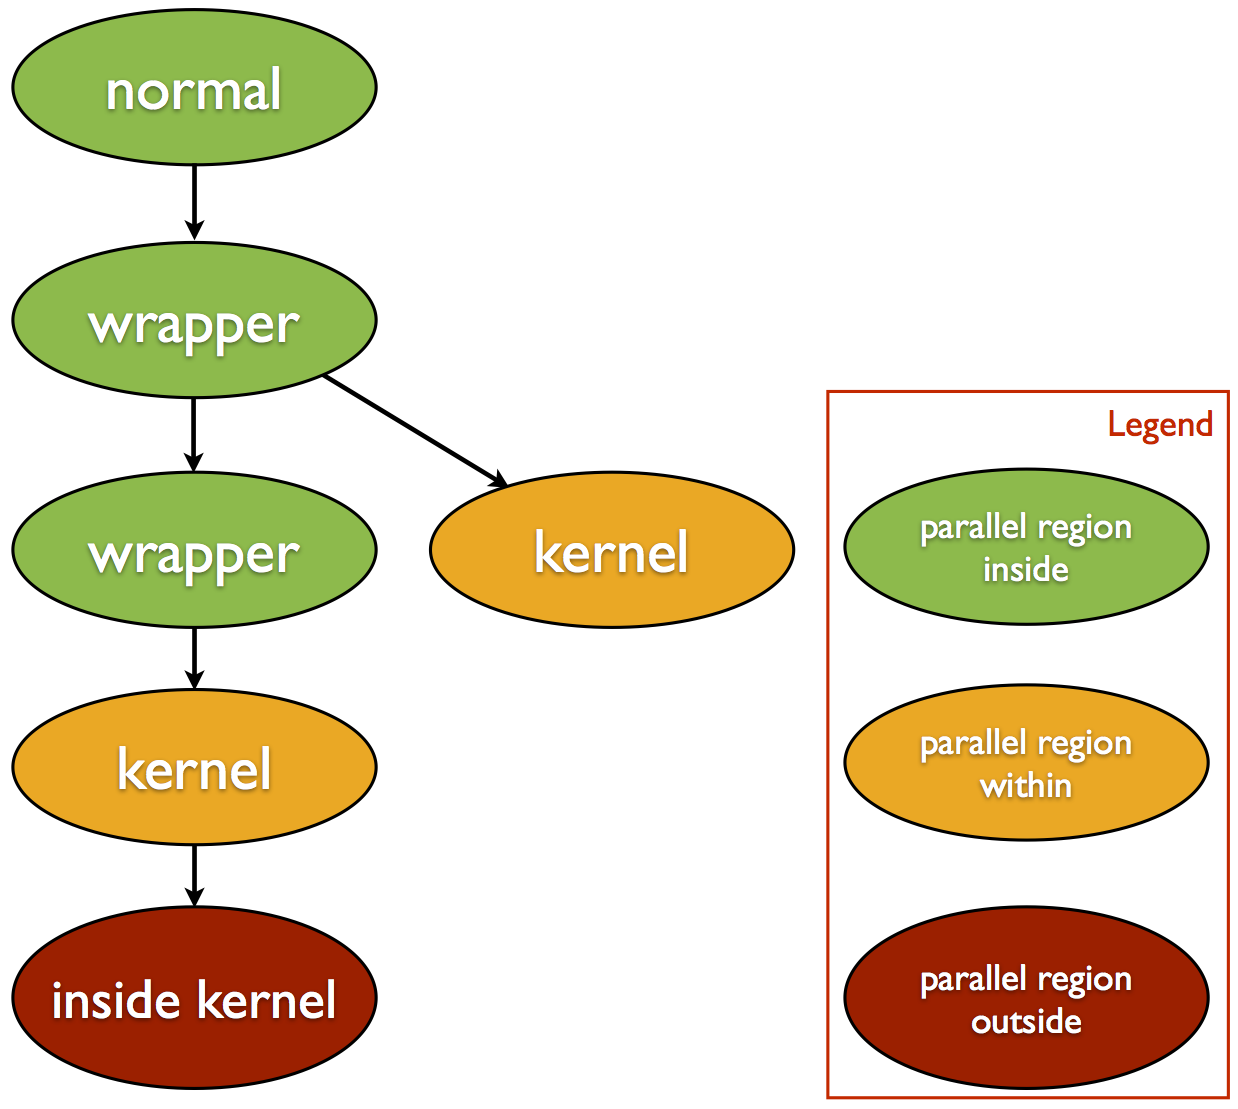
\includegraphics[width=7.5cm]{figures/subroutineTypes.png}
  \caption[Hybrid Fortran Subroutine Types]{Callgraph showing subroutine types with restrictions for GPU compilation.}
  \label{figure:subroutineTypes}
\end{figure}

\begin{enumerate}
 \item Hybrid Fortran has only been tested using free form Fortran 90 and Fortran 2003 syntax.
 \item Your free form files will need the f90 or F90 file endings for the Hybrid Fortran build system to pick them up (this is also recommended by Intel if you want to use their compiler).
 \item All pointers that are to touch the device need a specified intent and their domain / dimension setup needs to be specified within a domainDependant directive. See the \verb|diffusion3D| example for an example code on how to use pointers together with Hybrid Fortran.
 \item When using the CUDA Fortran backend, Hybrid Fortran only supports data parallel programming. In order to use reduce functions, it is recommended to either use BLAS/CUBLAS (see poisson2d solver example) or use the OpenACC backend together with \verb|@parallelRegion| directives and \verb|reduce| attributes.
 \item Because of OpenACC / CUDA Fortran restrictions, kernel- and inside kernel subroutines may not
  \begin{enumerate}
   \item contain symbols declared with the \verb|DATA| or \verb|SAVE| attribute.
   \item contain multiple parallel regions.
   \item be recursive.
   \item call other kernel subroutines.
   \item contain the \verb|recursive|, \verb|pure| and \verb|elemental| keywords.
   \item contain inline array initialisations. Static data initialisations are ideally being done outside the parallel loop, typically in \verb|init| subroutines for each module that are always executed on the CPU. \textbf{Hybrid Fortran} directives are not needed for code parts that are in no case to be executed on the GPU, however the compile time storage order needs to be be respected by using the same storage order macros as specified in the \ref{descr:domPP} and \ref{descr:accPP} attributes for the involved arrays. Alternatively you can specify \verb|@domainDependant| directives in these code parts, so HF will take over the storage order handling.
  \end{enumerate}
 \item Inside kernel subroutines called by kernel subroutines must reside in the same Fortran module as their caller.
 \item All symbols that are declared as domain dependant using \verb|@domainDependant| directives must be of \verb|integer|, \verb|real|, \verb|character| or \verb|logical| type (however any byte length within the Fortran 90/2003 specification is allowed). Hybrid Fortran doesn't currently have support for derived types containing data arrays that need to be copied onto the device. You can use derived types in host-only code however.
 \item Arrays that are declared as domain dependant using \verb|@domainDependant| directives may not appear in declaration lines with mixed domain dependance. Example:
 \begin{lstlisting}[name=exampleMixedOK, label=listing:exampleMixedOK, caption={This is ok.}]
 ..
 real(8), dimension(nz) :: a, b
 real(8), dimension(nz) :: c
 ..
 @domainDependant {domName(x), domSize(nx)}
 a, b
 @end domainDependant

 @domainDependant {domName(y), domSize(ny)}
 c
 @end domainDependant
 ..
 \end{lstlisting}

 \begin{lstlisting}[name=exampleMixedNotOK, label=listing:exampleMixedNotOK, caption={This is not ok.}]
 ..
 real(8) dimension(nz) :: a, b, c
 ..
 @domainDependant {domName(x), domSize(nx)}
 a, b
 @end domainDependant

 @domainDependant {domName(y), domSize(ny)}
 c
 @end domainDependant
 ..
 \end{lstlisting}
 \item All source files (h90\footnote{h90 is the file extension used for Hybrid Fortran source files.}, H90\footnote{H90 is the file extension used for Hybrid Fortran source files that contain same-file macro expansions.}, f90, F90) need to have distinctive filenames since they will be copied into flat source directories by the build system.
 \item Subroutines in h90 and H90 files need distinctive names for the entire source tree.
 \item Only subroutines are supported together with \textbf{Hybrid Fortran} directives, e.g. functions are not supported.
 \item Preprocessor directives that affect the Hybrid Fortran preprocessing (such as code macros) must be expandable from definitions within the same H90 file, i.e. imports are not followed. Use the H90 file suffix (instead of h90) in case you want to use macros in your code.
 \item If you use local module scalars inside a kernel subroutine, the wrapper subroutine must reside in the same module.
 \item Module scalars, when used in a kernel subroutine, will loose their constant characteristic on GPU. They therefore can't be used where a constant is required, such as in a \verb|case| statement. (They do work as a dimension specifier for automatic arrays however.)
 \item I/O statements such as \verb|read| or \verb|write| and \verb|STOP| statements are not possible inside GPU parallel regions, except for emulated mode. \verb|print| is however supported.
\end{enumerate}

In general, since
\begin{enumerate}
  \item GPU execution currently requires subroutine calls to be inlined and
  \item the number of registers per GPU Streaming Multiprocessor is limited
\end{enumerate}
it is best to split deep callgraphs and large computations into multiple smaller kernels (i.e. \verb|@parallelDomain{ appliedTo(GPU), ..}|).

\clearpage
\section{Device Data Handling} \label{sec:deviceDataHandling}
The goal of device data handling is to hide and abstract code that is only necessary for the CUDA execution path. \textbf{Hybrid Fortran} works similarly to OpenACC in that respect. For all non-scalars that are marked as domain dependant using the \verb|@domainDependant| directive, the following rules apply with respect to device data in case of GPU compilation:
\begin{enumerate}
  \item If the current subroutine contains calls to kernel subroutines and the domain dependant symbol is declared using the \verb|intent(in)| or \verb|intent(inout)| statement, a device version of the symbol will be allocated and its content will be copied to that device array at the beginning of the subroutine.
  \item If the current subroutine contains calls to kernel subroutines and the domain dependant symbol is declared using the \verb|intent(out)| or \verb|intent(inout)| statement, a device version of the symbol will be allocated and set to zero and the device array's content will be copied to the original array at the end of the subroutine.
  \item If the domain dependant symbol is local for this subroutine, it will be allocated as a device symbol and its content will be set to zero at the beginning of the subroutine.
  \item In case the domain dependant directive contains an \verb|attribute(present)| statement, no data will be copied and the original symbol will be declared as a device symbol.
  \item In case the domain dependant directive contains an \verb|attribute(transferHere)| statement, the data will always copied over to the device, following the specified intents (as in (1), (2)).
\end{enumerate}

\subsection{Module Data}
Using the following guidelines, Hybrid Fortran is able to manage your imported module data to be copied to and from the device.
\begin{enumerate}
 \item After the specification part of your module, add \verb|@domainDependant| directives and include all arrays that need to be touched by your parallel regions.
 \item In case your module data arrays are allocatable (which is probably the case if your problem dimensions are runtime defined), you cannot use \verb|attribute(autoDom)|. Instead, use the \verb|domName| and \verb|domSize| attributes to specify the domain setup. You may use runtime defined scalar variables (e.g. \verb|nx|, \verb|i|, ...) within this specification as long as these variables are always defined within the parallel regions that use these arrays. These runtime variables do \textbf{not} need to be imported into the declaring module.
 \item Specify \verb|attribute(host)| for all these arrays in the module specification.
 \item In the module data consuming kernel subroutine, simply import the data with \verb|use| statements (please note that Hybrid Fortran cannot parse multiline \verb|use| statements at this point) and specify them also inside the corresponding \verb|domainDependant| directive. You may use \verb|attribute(autoDom)| there, since Hybrid Fortran will use the domain information that you provide in the module specification. The data handling at this point follows the same rules as locally declared arrays (see above) - so make sure that you use \verb|attribute(present)| and \verb|attribute(transferHere)| if you have multiple kernel subroutines that touch the same data.
\end{enumerate}

\clearpage
\section{Feature Comparison between Hybrid Fortran and OpenACC} \label{sec:featureComparisonFrameworks}

The following table gives an overview over the differences between OpenACC and the \textbf{Hybrid Fortran} framework.

\begin{table}[htpb]
  \centering
  \footnotesize
  \begin{tabular}{l|c|c|l}
    Feature & OpenACC & Hybrid & Comments \\
    & & Fortran 90 & \\
    \hline \hline
    Enables close to fully optimized  & & \checkmark & CUDA Fortran implementation \\
    Fortran code for GPU execution & & & available, which has equal or better \\
    & & & performance than OpenACC in all \\
    & & & cases known to us \\
    \hline
    Enables close to fully & & \checkmark & Storage order abstraction as well \\
    optimized Fortran code & & & as allowing both coarse grained \\
    for CPU execution & & & as well as fine grained parallelization \\
    & & & leads to this result. \\
    \hline
    Automatic device data & \checkmark & \checkmark & \\
    copying & & & \\
    \hline
    Allows adjusted looping & & \checkmark & \\
    patterns for CPU and & & & \\
    GPU execution & & & \\
    \hline
    Allows changing the & & \checkmark & \\
    looping patterns with & & & \\
    minimal adjustments in & & & \\
    user code & & & \\
    \hline
    Handles compile time & & \checkmark & \\
    defined storage order & & & \\
    \hline
    Allows to adapt & & \checkmark & Details, see section \ref{sub:switchImplementation} \\
    for other technologies & & & \\
    without changing the user & & & \\
    code (e.g. switching to & & & \\
    OpenCL) & & & \\
    \hline
    Allows arbitrary access & \checkmark & \checkmark &  \\
    patterns in parallel & & & \\
    domains & & & \\
    & & & \\
    & & & \\
    \hline
    Allows multiple parallel & \checkmark & (\checkmark) & HF: Only OpenACC backend. \\
    regions per subroutine & & & \\
    \hline
    Generated GPU code remains & & \checkmark & OpenACC compiles to CUDA C \\
    easily human & & & (PGI), introduces new \\
    readable & & & functions for device kernels. \\
    & & & Hybrid Fortran can translate to \\
    & & & CUDA Fortran, code remains \\
    & & & easily readable.\\
    \hline
    Allows debugging of & \checkmark & \checkmark & \\
    device data & & & \\
    \hline
    Framework Sourcecode & & \checkmark & \\
    available & & & \\
    \hline
  \end{tabular}
  \caption{Feature Comparison OpenACC vs. Hybrid Fortran}
  \label{table:featureComparisonFrameworks}
\end{table}